\section{}
Verify the results in Fig. \ref{fig:Q4ProblemDiagram} by employing 
\begin{equation*}
    \sigma_{\theta} = \frac{1}{2} \sigma_o \left[\left(1+\frac{a^2}{r^2}\right) - \left(1 + \frac{3a^4}{r^4}\cos{2\theta} \right) \right]
\end{equation*}

\begin{figure}[h]
    \centering
    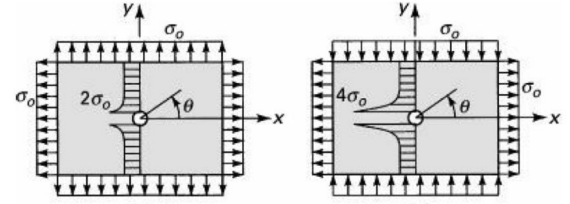
\includegraphics[width=0.5\linewidth]{Questions/Figures/Q4ProblemDiagram.png}
    \caption{Problem diagram for Question 4.}
    \label{fig:Q4ProblemDiagram}
\end{figure}

\begin{figure}[h]
    \centering
    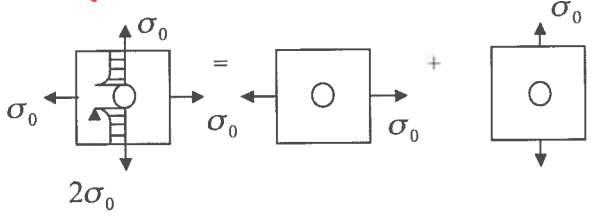
\includegraphics[width=0.5\linewidth]{Questions/Figures/Q4SuperpositionDiagram.png}
    \caption{Superposition of stresses for Question 4.}
    \label{fig:Q4SuperpositionDiagram}
\end{figure}

\subsection{}
First the axial load in the $x$ direction will be considered. The maximum is
\begin{align*}
    (\sigma_\theta)_{\text{max}} = 3 \sigma_o, \quad \theta = \pm \pi/2 \\
\end{align*}
Secondly, in the $y$ direction,
\begin{align*}
    (\sigma_\theta)_{\text{min}} = -\sigma_o, \quad \theta = \pm \pi/2
\end{align*}
Since $x$ and $y$ are offset by $90^\circ$, the maximum of $x$ adds to the minimum of $y$. Therefore, we can verify
\begin{empheq}[box=\fbox]{align*}
    \sigma_r &= \tau_{r\theta} 0, \text{by boundary conditions} \\
    \sigma_\theta &= (3 + (-1)) \sigma_o = 2 \sigma_o
\end{empheq}

\subsection{}
In the $y$ direction, the direction of $\sigma_o$ is reversed. The maximum and minimum become
\begin{align*}
    (\sigma_\theta)_{\text{min}} = \sigma_o, \quad \theta = 0, \pi
\end{align*}
Again, since $x$ and $y$ are offset by $90^\circ$, so
\begin{empheq}[box=\fbox]{align*}
    \sigma_r &= \tau_{r\theta} 0, \text{by boundary conditions} \\
    \sigma_\theta &= (3 + 1) \sigma_o = 4 \sigma_o
\end{empheq}